\section{Decay Time}
\label{sec:ana_time}

The theoretical model of the decay time of \BstoJpsiKK{} decays is distorted by two experimental effects; the uncertainty in the time
measurement (\emph{resolution}) and the efficiency of the measurement (\emph{acceptance}) as a function of time. As discussed in
Section~\ref{subsec:intro_LHCb_Jpsiphi}, the resolution is roughly 0.05\unitsp{}ps. The resolution model is presented in
Section~\ref{subsec:ana_time_res}. The decay-time measurement is affected by non-trivial acceptance effects from both the trigger and
reconstruction processes, which will be discussed in Section~\ref{subsec:ana_time_acc}.


%%%%%%%%%%%%%%%%%%%%%%%%%%%
\subsection{Resolution}
\label{subsec:ana_time_res}
%%%%%%%%%%%%%%%%%%%%%%%%%%%

The uncertainty in the decay-time measurement causes a difference between the measured decay time and the true decay time. This difference
is a random variable and the resulting measured time distribution is a smeared version of the underlying true distribution. For the
oscillatory $\cDms$ and $\sDms$ functions in the differential decay rate this smearing causes a decrease, or \emph{dilution}, of the
oscillation amplitude. As described in Section~\ref{subsec:pheno_equations_approx}, the main sensitivity for the CP-violation parameters
originates from the oscillation terms and hence a diluted oscillation amplitude reduces the statistical precision of the estimates for
these parameters.

For each decay the decay-time uncertainty is estimated by propagating the uncertainties in the positions of the primary and secondary
vertices and particle momenta, as discussed in Section~\ref{subsec:intro_LHCb_Jpsiphi}. The distribution of this estimate ($\sigmat$) is
shown in Figure~\ref{fig:sigmat}. For each decay, the probability for the measured decay time to deviate by a given amount from the true
decay time is approximately described by a Gaussian distribution with width $\sigmat$.
\begin{figure}[htbp]
  \centering
  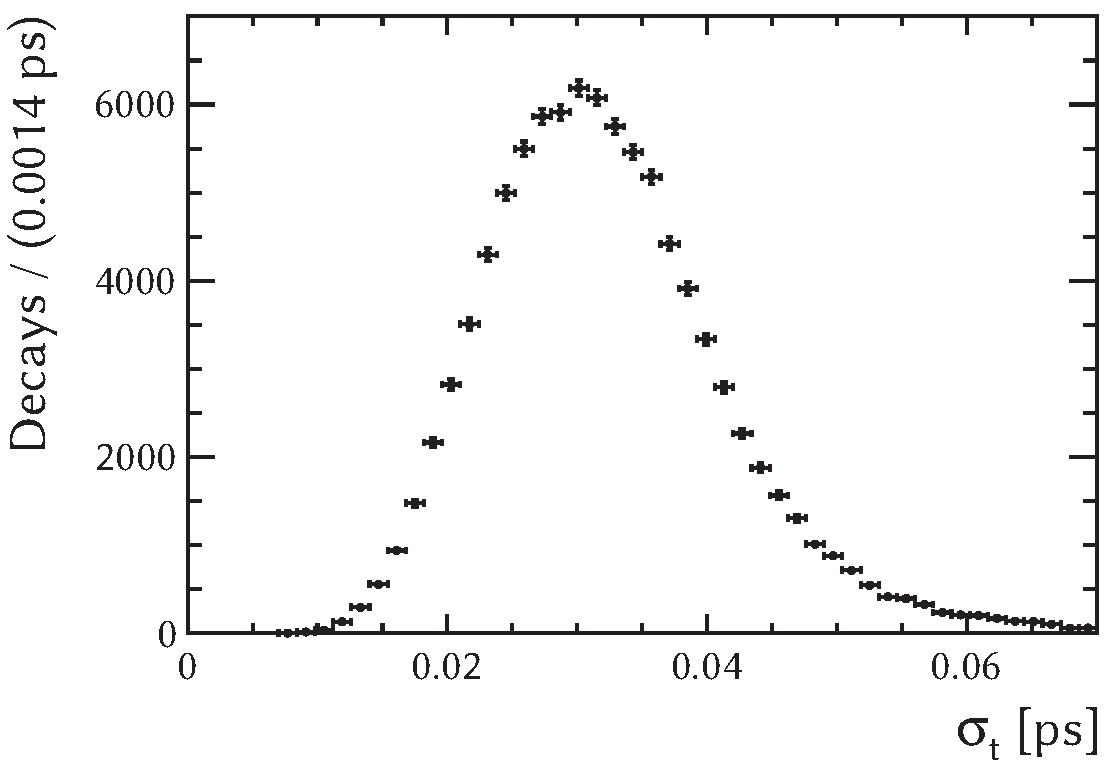
\includegraphics[width=0.5\textwidth]{graphics/analysis/sigmat}
  \caption{Distribution of \BstoJpsiKK{} signal decays in the estimated decay-time uncertainty.}
  \label{fig:sigmat}
\end{figure}

Decay-time resolution is included in the model for the signal decay by convolving the theoretical model with the model for the difference
between the measured time and the true time. This convolution is the integral of the two-dimensional PDF of the true and measured decay
times over all possible values of the former:
\begin{equation}
  P_\text{meas}(t_\text{meas}, \Omega)
    \equiv \int_0^\infty \ud t_\text{true}\, R(t_\text{meas} - t_\text{true}|\sigmat)\, P_\text{true}(t_\text{true}, \Omega)\ ,
\end{equation}
where $R$ is the PDF for the difference between the measured and true times, or the \emph{resolution model}. The resolution model is
conditional on $\sigmat$., i.e. normalized with respect to decay time for each individual value of $\sigmat$.

Although the resolution model is approximated by a Gaussian PDF with width $\sigmat$, a more sophisticated model is required to describe
the resolution in the PDF with sufficient precision. The model is a sum of two Gaussian PDFs with a common, non-zero mean and a width that
depends quadratically on $\sigmat$. The width of the first Gaussian PDF is approximately equal to $\sigmat$, while the width of the second
Gaussian PDF is roughly a factor two larger.

The double-Gaussian model is based on and validated with both simulated \BstoJpsiKK{} decays and prompt background decay candidates. Since
all tracks of prompt background candidates originate from the primary vertex, their ``true'' decay time is equal to zero and the
distribution of measured decay times is essentially the resolution model. Studies of the model and its parameters are described in detail
in references~\cite{Aaij:2015} and \cite{LHCb-ANA-2014-039}. The values of the resolution parameters are fixed in the fit of decay time and
angles. Uncertainties in the parameter values are propagated after the fit and accounted for as systematic uncertainties (see
Section~\ref{sec:result_syst}).


%%%%%%%%%%%%%%%%%%%%%%%%%%%
\subsection{Acceptance}
\label{subsec:ana_time_acc}
%%%%%%%%%%%%%%%%%%%%%%%%%%%

To account for the efficiencies of the decay-candidate reconstruction and selection processes, the PDF is multiplied by an acceptance
function and re-normalized to create a new PDF. The acceptance is is modelled as a product of two functions of decay time and one function
of decay angles. The angular part will be discussed in Section~\ref{sec:ana_angles}. This section describes the two decay-time functions.

\subsubsection{Track-Reconstruction Acceptance}
The first part of the non-trivial acceptance in decay time originates from an inefficiency in the reconstruction of particle tracks. This
efficiency decreases for increasing distance between the track and the proton beams. Since the distance between the primary and secondary
vertex and, therefore, the decay time are correlated with the distance between the four \BstoJpsiKK{} tracks and the beams, the efficiency
also decreases with increasing decay time.

In the measurement presented here the track-reconstruction acceptance is modelled by an exponential function in \emph{true} decay time. The
advantage of this model is that its implementation in the model of the decay-time distribution is straightforward. An exponential function
can be absorbed in the $\eGst$ factor of the differential decay rate (Equation~\ref{eq:angCoefs}):
\begin{equation}
  \eGst \longrightarrow e^{\beta\,t}\,\eGst = e^{-(\Gs-\beta)\,t} \equiv e^{-\Gs^\text{eff}\,t}\ ,
\end{equation}
where $\beta$ is the parameter that quantifies the rate at which the efficiency changes as a function of decay time. The parameter
$\Gs^\text{eff}$\textequiv$\Gs$\textminus$\beta$ can now be included in the model in the place of the parameter $\Gs$.

The parameter $\beta$ has been determined by a combination of studies with real and simulated data~\cite{LHCb-ANA-2014-039}. Because of
changes in the online reconstruction algorithms between the 2011 and 2012 runs and the different proton-collision energies in these
periods, the corresponding values of $\beta$ are evaluated separately: $\beta_\text{2011}$\texteq\mbox{\tm0.0090\textpm0.0022\unitsp\invps}
and $\beta_\text{2012}$\texteq\mbox{\tm0.0124\textpm0.0019\unitsp\invps}. These values have to be compared with
$\Gs$\textapprox0.66\unitsp\invps.

Although there is no sensitivity in the \BstoJpsiKK{} data to the parameters $\Gs$, $\beta_\text{2011}$, and $\beta_\text{2012}$
separately, the value of $\Gs^\text{eff}$ can be determined in the fit of decay time separately for the 2011 and 2012 periods.
Reparameterizing, there is sensitivity for the combinations $\Gs$\textminus$\tfrac{1}{2}(\beta_\text{2011}$\textplus$\beta_\text{2012})$
and $\beta_\text{2012}$\textminus$\beta_\text{2011}$.

To combine the information on the difference between the two $\beta$ values with the externally determined values, the $\beta$ parameters
are varied with constraints in the time and angular fit. These constraints are implemented by adding a parabolic term to the NLL of the
form $\frac{1}{2\hat{\sigma}^2}(\beta-\hat{\beta})^2$ for each parameter, where the external value is denoted by $\hat{\beta}$ and the
external uncertainty by $\hat{\sigma}$. Because these external constraints are much tighter than the constraints from the \BstoJpsiKK{}
data, the values that are estimated in the fit are comparable to the external values:
$\beta_\text{2011}$\texteq\mbox{\tm0.0086\textpm0.0021\unitsp\invps} and
$\beta_\text{2012}$\texteq\mbox{\tm0.0127\textpm0.0018\unitsp\invps}.

There are some limitations to this model of the track-reconstruction acceptance. The model is implemented for true decay time, whereas the
external values of the $\beta$ parameters were evaluated with the measured decay time. In this measurement, this is assumed to be a good
approximation, because the time scale of the variations in the model is much larger than the resolution. That is,
$\beta^{-1}$\textapprox\mbox{\tenpow{2}\unitsp{}ps}\textgg\mbox{0.05\unitsp{}ps}.

Also the model itself is an approximation. As was shown in reference~\cite{LHCb-ANA-2014-039}, the shape of the acceptance is better
described by the function 1\textplus$\beta\,t$\textplus$\beta'\,t^2$ than by $e^{\beta\,t}$\textapprox1\textplus$\beta\,t$. A systematic
uncertainty in the parameter estimates corresponding to the assumption of the shape $e^{\beta\,t}$ is estimated in
Section~\ref{sec:result_syst}.

\subsubsection{Trigger Acceptance}
As described in Section~\ref{subsec:ana_bkgSub_sel}, there are also trigger requirements that introduce non-trivial acceptance effects in
decay time. The shapes of the acceptance functions corresponding to the decay-time biasing trigger categories are determined relative to
the shapes of the unbiased categories, which have a uniform acceptance function.

The shape of the trigger acceptance is described in bins of decay time. For each bin, numbers of decays are counted in the different
trigger categories to determine the relative efficiency in the bin. To also include information on the exponential shape of the decay in
the resulting binned acceptance function, the decay counts are varied in the fit of decay time and angles.

Since normally only the shape of the differential decay rate in time and angles is determined in the fit, additional terms need to be
included in the NLL to count decays in the different trigger categories. For unweighted decays the PDF for the number of decays in a
category would be a Poisson distribution, which is proportional to $\nu^n\,e^{-\nu}$, where $n$ is the observed number of decays and $\nu$
the parameter for the expected number of decays. This PDF would give an additional NLL term of $\nu$\textminus$n\,\ln\nu$. However, because
each decay candidate is counted with its signal weight, this term is modified to obtain the correct uncertainty on the parameter $\nu$ from
a maximum-likelihood fit.

The variable $n$ in the Poissonian NLL term is replaced by the sum of the decay-candidate weights and the NLL term is multiplied by a
factor that also depends on the weights:
\begin{equation}
  \label{eq:weightPoisson}
  \frac{\sum w}{\sum w^2}\left( \nu - \ln\nu\,\sum w \right)\ ,
\end{equation}
where $\sum w$ is the sum of the decay weights and $\sum w^2$ the sum of the squared decay weights. This function reaches its minimum at
$\nu$\texteq$\sum w$, so the estimated value for $\nu$ in a maximum-likelihood fit with only this function would be the sum of the decay
weights. The inverse of the second derivative of the function, from which the uncertainty in $\nu$ is estimated, is given by $\sum w^2$
instead of $\sum w$ for an unmodified Poisson term. The former number is equal to the variance that is expected when counting weighted
decay candidates.

Decays are categorized with the sets of HLT selection criteria discussed in Section~\ref{subsec:ana_bkgSub_sel}. For the purpose of
determining selection efficiencies, the combination of the HLT1 requirements and the part of the selection requirements that the two HLT2
selections have in common is termed \emph{phase 1}. The subsequent \emph{phase 2} then only consists of the minimum-DLS requirement in the
biased HLT2 selection and the uniform reduction of decays in the unbiased HLT2 selection.

Decays that pass the selection requirements of phase 1 are selected by only the biased HLT1 requirements, by only the unbiased HLT1
requirements, or by both sets. Only the shape of the acceptance in decay time is required for the fit, which is assumed to be uniform for
the unbiased phase-1 (HLT1) selection. The shape of the biased phase-1 selection is determined relative to the unbiased shape by
calculating the ratio of the numbers of biased and unbiased decays in each bin of decay time.

Since the uniform selection of decays in the unbiased HLT2 selection does not depend on any of the properties of a decay, the biased and
unbiased phase-2 selections are independent. That is, the efficiency of the minimum-DLS requirement does not depend on whether a decay was
selected by the uniform selection and vice versa. As a result, decays selected by the unbiased phase-2 requirements are representative for
the full sample of events and the biased phase-2 efficiency is given by the fraction of unbiased decays that was also selected by the
minimum-DLS requirement.

Implementing these concepts in an acceptance model for the fit, six trigger categories are defined based on whether of not decays were
selected by the unbiased set of requirements in phase 1, by the minimum-DLS requirement in phase 2, and by the uniform selection in phase
2. In principle this gives a total of eight categories, but in two of these no decays are selected by construction, because they are
neither selected by the minimum-DLS requirement nor by the uniform phase-2 selection. If a decay is not selected by the unbiased phase-1
(HLT1) selection it can still be selected (exclusively) by biased phase-1 (HLT1) selection, which leaves six non-empty categories. The
categories are listed in Table~\ref{tab:triggerCats}.
\begin{table}[tbp]
  \centering
  \caption{Definition of the six trigger categories that are used to determine the shape of the decay-time acceptance
           introduced by the HLT.
           For each category it is indicated if the decays it contains are selected by the unbiased phase-1 selection (``p1 unb.''),
           by the unbiased phase-2 selection (``p2 unb.''), and by the biased phase-2 selection (``p2 bias.'').
           The ratio of the exclusively-biased and unbiased phase-1 efficiencies is given by $r_\text{1}$,
           the efficiency of the unbiased phase-2 selection by $\varepsilon_\text{2U}$,
           and the efficiency of the biased phase-2 selection by $\varepsilon_\text{2B}$.
           The number of decays that passes the unbiased phase-1 selection is given by $\nu_\text{1U}$.}
  \label{tab:triggerCats}
  \begin{tabular}{ccccl}
    \hline
    category  &  p1 unb.  &  p2 unb.  &  p2 bias.  &  number of decays  \\
    \hline
    1  &  *  &  *  &  *
       &  $\varepsilon_\text{2U}\, \varepsilon_\text{2B}\, \nu_\text{1U}$  \\
    2  &  *  &     &  *
       &  $(1-\varepsilon_\text{2U})\, \varepsilon_\text{2B}\, \nu_\text{1U}$  \\
    3  &  *  &  *  &
       &  $\varepsilon_\text{2U}\, (1-\varepsilon_\text{2B})\, \nu_\text{1U}$  \\
    4  &     &  *  &  *
       &  $r_\text{1}\, \varepsilon_\text{2U}\, \varepsilon_\text{2B}\, \nu_\text{1U}$  \\
    5  &     &     &  *
       &  $r_\text{1}\, (1-\varepsilon_\text{2U})\, \varepsilon_\text{2B}\, \nu_\text{1U}$  \\
    6  &     &  *  &
       &  $r_\text{1}\, \varepsilon_\text{2U}\, (1-\varepsilon_\text{2B})\, \nu_\text{1U}$  \\
    \hline
  \end{tabular}
\end{table}

By counting decays in the fit in each of the six trigger categories the parameters in the last column of Table~\ref{tab:triggerCats} can be
determined. The expression for the number of decays in the category takes the place of $\nu$ in Equation~\ref{eq:weightPoisson} and the
parameters in the expression are varied in the fit.

The ratio of the phase-1 exclusively-biased and unbiased efficiencies, $r_\text{1}$, is effectively determined from the respective ratios
of the numbers of decays in categories 4, 5, and 6 and the categories 1, 2, and 3. The distributions of decays over categories 1, 2, and 3
and over categories 4, 5, and 6 determine the value of the number of decays the pass the unbiased phase-1 selection, $\nu_\text{1U}$, the
efficiency of the phase-2 unbiased selection, $\varepsilon_\text{2U}$, and the efficiency of the  phase-2 biased selection,
$\varepsilon_\text{2B}$.

Because the efficiency of the biased phase-2 selection is high, 96--98\%, the not-biased phase-2 categories 3 and 6 contain few decays. For
this reason these two categories are merged and only the sum of weights of both categories is parameterized. This reduces the sensitivity
to the parameter $r_\text{1}$, which is only estimated with the ratio of categories 4 and 1 and the ratio of categories 5 and 2.

Although the sums of weights are evaluated for all available decays, the NLL for the fit of decay time and angles is built with only biased
phase-2 decays. The PDF is multiplied by a factor $\varepsilon_\text{2B}$ for unbiased phase-1 decays (the sum of categories 1 and 2) and a
factor $r_\text{1}\, \varepsilon_\text{2U}$ for exclusively-biased phase-1 decays (the sum of categories 4 and 5). This simplifies the
measurement, because no NLL is constructed for the remaining biased phase-2 decays. Almost no sensitivity to parameter estimates is lost,
because of the small fraction of decays in these remaining categories.

The above description of the HLT acceptance function assumes that the efficiencies for the phase-2 selection are independent of the phase-1
category. That is, the values of the parameters $\varepsilon_\text{2U}$ and $\varepsilon_\text{2B}$ are equal for categories 1--3 and 4--6.
This is based on the assumption that, at each point in decay time, the minimum-DLS requirement in the biased phase-2 selection is
independent of any of the phase-1 requirements.

To test these assumptions the fit is repeated with an alternative acceptance model. In the alternative model, the unbiased phase-1
categories (1--3) are unchanged and are give estimates of the phase-2 efficiencies for unbiased phase-1 decays, $\varepsilon_\text{2U|1U}$
and $\varepsilon_\text{2B|1U}$. Instead of counting decays in all exclusively-biased phase-1 categories (4--6), only the total sum of
weights for phase-2 biased decays is used in the fit (the sum of categories 4 and 5). This sum is parameterized by
$r_\text{1}\, \varepsilon_\text{2B|1exclB}\, \nu_\text{1U}$.

Only the product $r_\text{1}\, \varepsilon_\text{2B|1exclB}$ can be estimated in this model and not these parameters separately, but this
suffices, since it is exactly this product that is required in the time and angular PDF. Although the removal of assumptions in the
alternative model leads to slightly larger statistical uncertainties on the efficiency parameters, the results with the two acceptance
models are compatible.

\begin{figure}[htbp]
  \centering
  \begin{subfigure}{0.49\textwidth}
    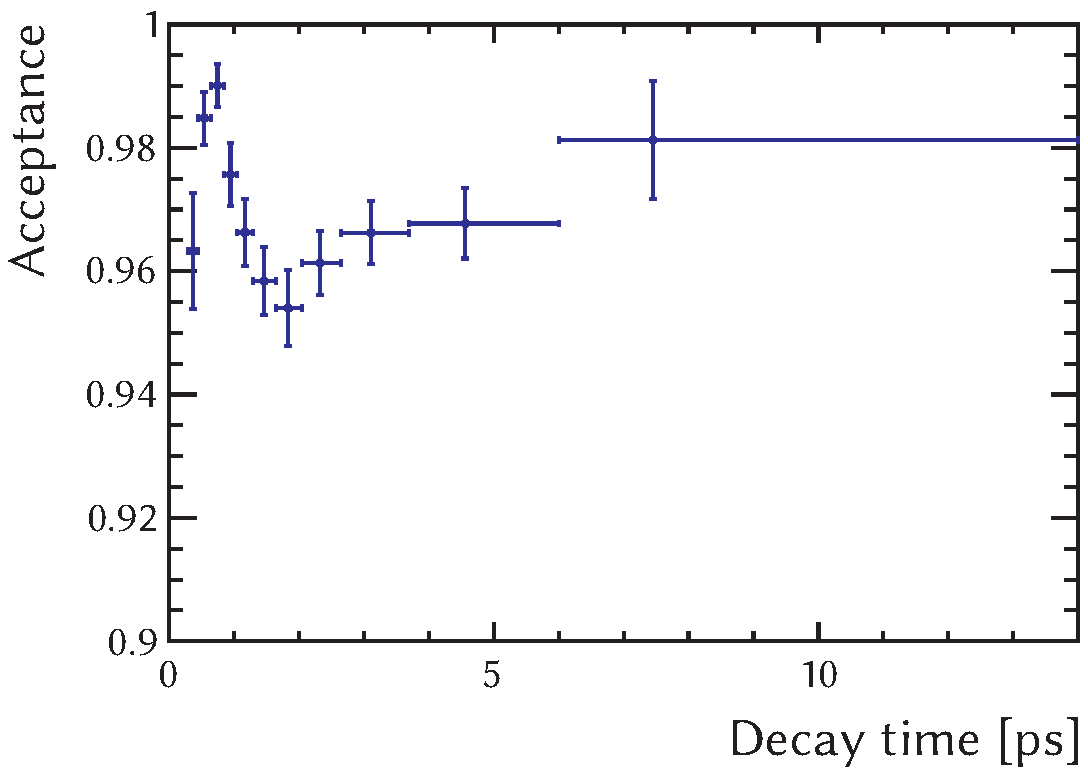
\includegraphics[width=\textwidth]{graphics/analysis/trigTimeAcc_2011_UB}
    \caption{}
    \label{fig:trigAcc_2011_UB}
  \end{subfigure}%
  \hfill%
  \begin{subfigure}{0.49\textwidth}
    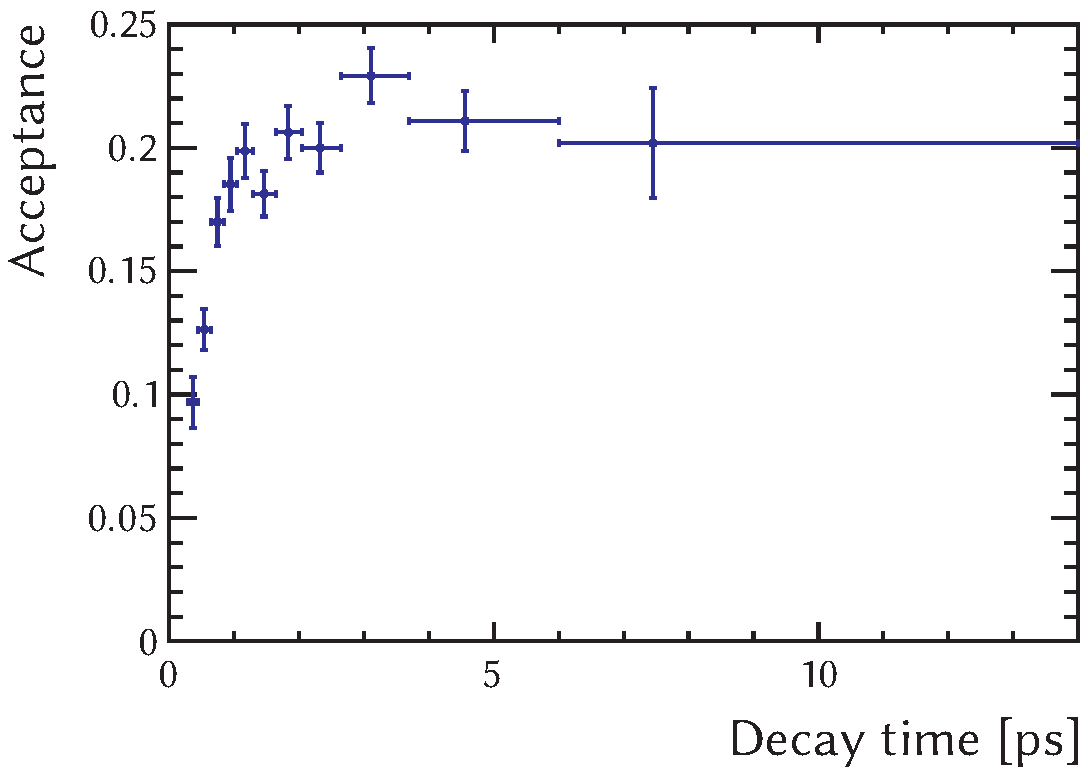
\includegraphics[width=\textwidth]{graphics/analysis/trigTimeAcc_2011_exclB}
    \caption{}
    \label{fig:trigAcc_2011_exclB}
  \end{subfigure}

  \vspace*{0.02\textwidth}
  \begin{subfigure}{0.49\textwidth}
    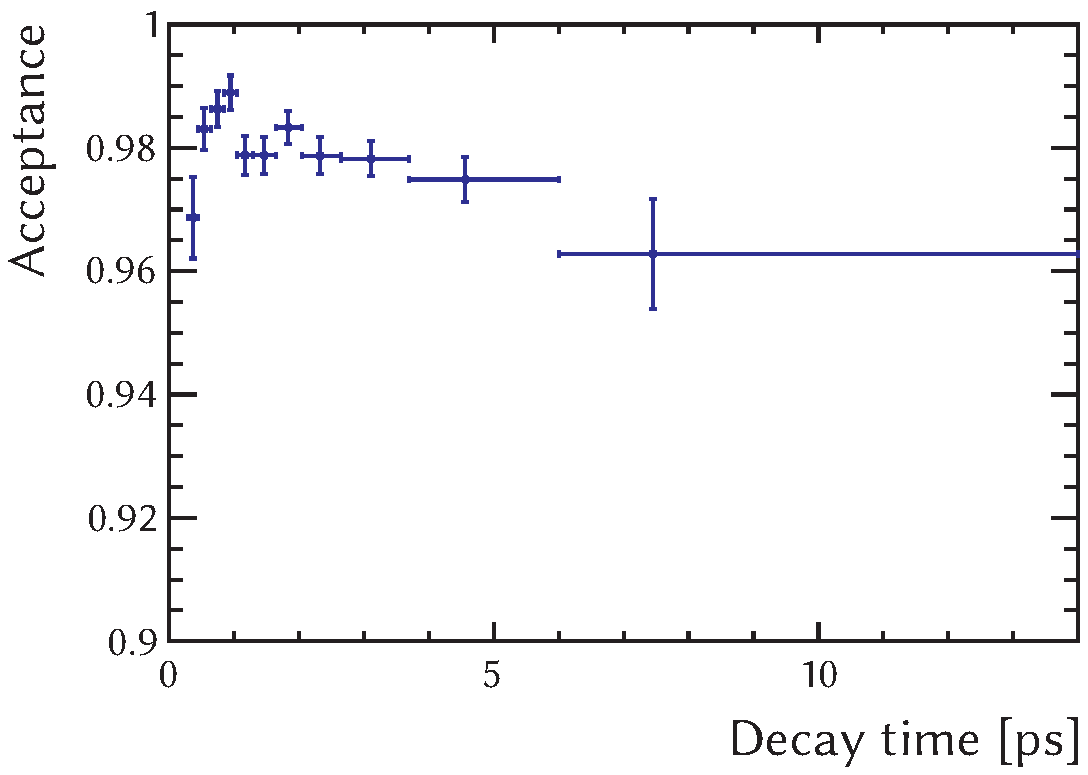
\includegraphics[width=\textwidth]{graphics/analysis/trigTimeAcc_2012_UB}
    \caption{}
    \label{fig:trigAcc_2012_UB}
  \end{subfigure}%
  \hfill%
  \begin{subfigure}{0.49\textwidth}
    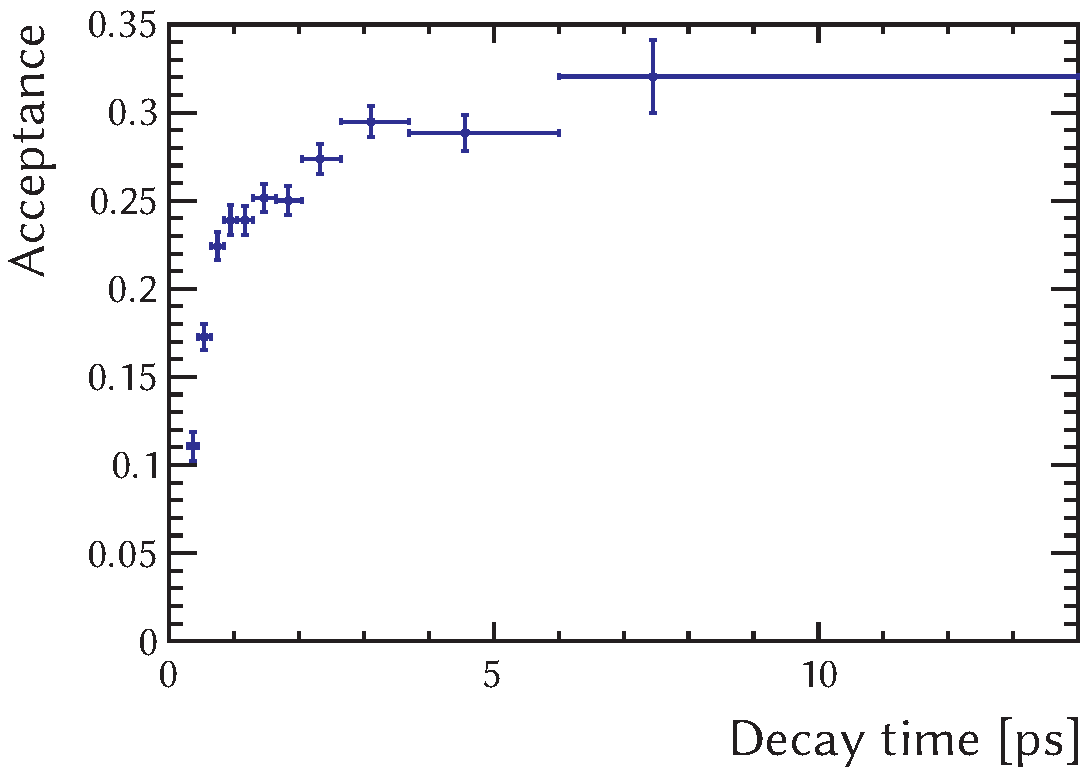
\includegraphics[width=\textwidth]{graphics/analysis/trigTimeAcc_2012_exclB}
    \caption{}
    \label{fig:trigAcc_2012_exclB}
  \end{subfigure}
  \caption{Trigger acceptance in bins of decay time for (a, b) the 2011 run and (c, d) the 2012 run
           and for (a, c) the unbiased phase-1/biased phase-2 selection and (b, d) the exclusively-biased phase-1/biased phase-2 selection.
           Notice that the efficiency range of the unbiased phase-1/biased phase-2 graphs is 90--100\%.
           Because the absolute efficiency of the phase-1 selections is unknown, the scales of the efficiencies
           in the graphs are given with respect to the efficiency of the unbiased phase-1 selection.}
  \label{fig:trigAcc}
\end{figure}

The shapes of the HLT-acceptance functions that are used in the time and angular model are shown in Figure~\ref{fig:trigAcc} for both the
2011 and 2012 runs. The scale of the vertical axes was divided by the efficiency of the unbiased phase-1 selection, which is undetermined.
Whereas 40 decay-time bins are used for the nominal measurement, only 11 bins are used for these plots to reduce statistical fluctuations.

A sharp rise in efficiency, or \emph{turn-on}, is visible in all acceptance curves just above the minimum decay time of 0.3\unitsp{}ps.
After the turn-on, a dip in the efficiency occurs around 2\unitsp{}ps for the unbiased phase-1 curve for 2011
(Figure~\ref{fig:trigAcc_2011_UB}). This dip was caused by an inefficiency in the vertex reconstruction, which was reduced in 2012
(Figure~\ref{fig:trigAcc_2012_UB}). The exclusively-biased phase-1 curves (Figures~\ref{fig:trigAcc_2011_exclB} and
\ref{fig:trigAcc_2012_exclB}) have a slower turn-on than the unbiased phase-1 curves, because of the decay-time biasing requirements on
muon tracks in HLT1.
